\documentclass{beamer}

\usepackage[utf8]{inputenc}
\usepackage{bm}

%Information to be included in the title page:
\title{Utilization of Instance Relationship in Knowledge Distillation}
\author{Zhang Yuan}
\date{2020.07.03}

\usefonttheme[onlymath]{serif}
\begin{document}

\frame{\titlepage}

\begin{frame}
\frametitle{Review}
Vanilla KD \\
$L_{KD}=\sum\limits_{x_i\in \mathcal X}{\textrm{H}(\textrm{softmax}(\frac{f_T(x_i)}{t}), \textrm{softmax}(\frac{f_S(x_i)}{t}))}$\\
$L_{GT}=\sum\limits_{x_i\in \mathcal X}{\textrm{H}(\textrm{one-hot}(y_i),\textrm{softmax}(f_S(x_i)))}$\\
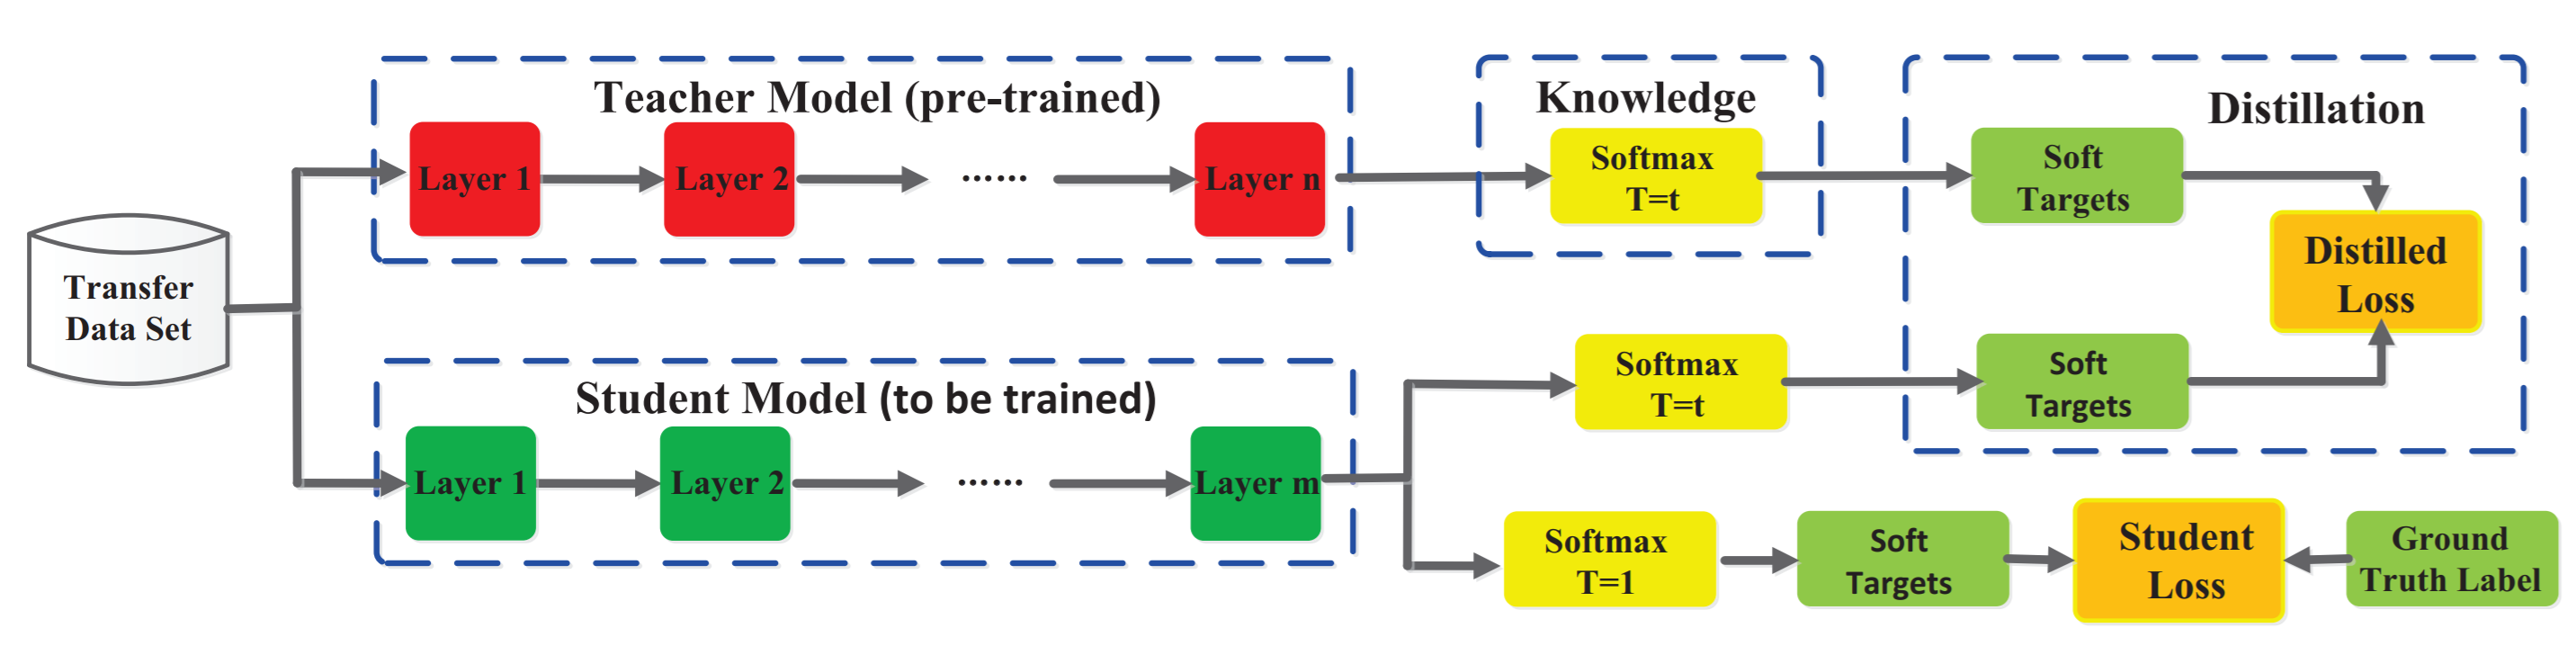
\includegraphics[width=0.8\textwidth]{hinton_kd.png} \\
Use Inner Layers \\
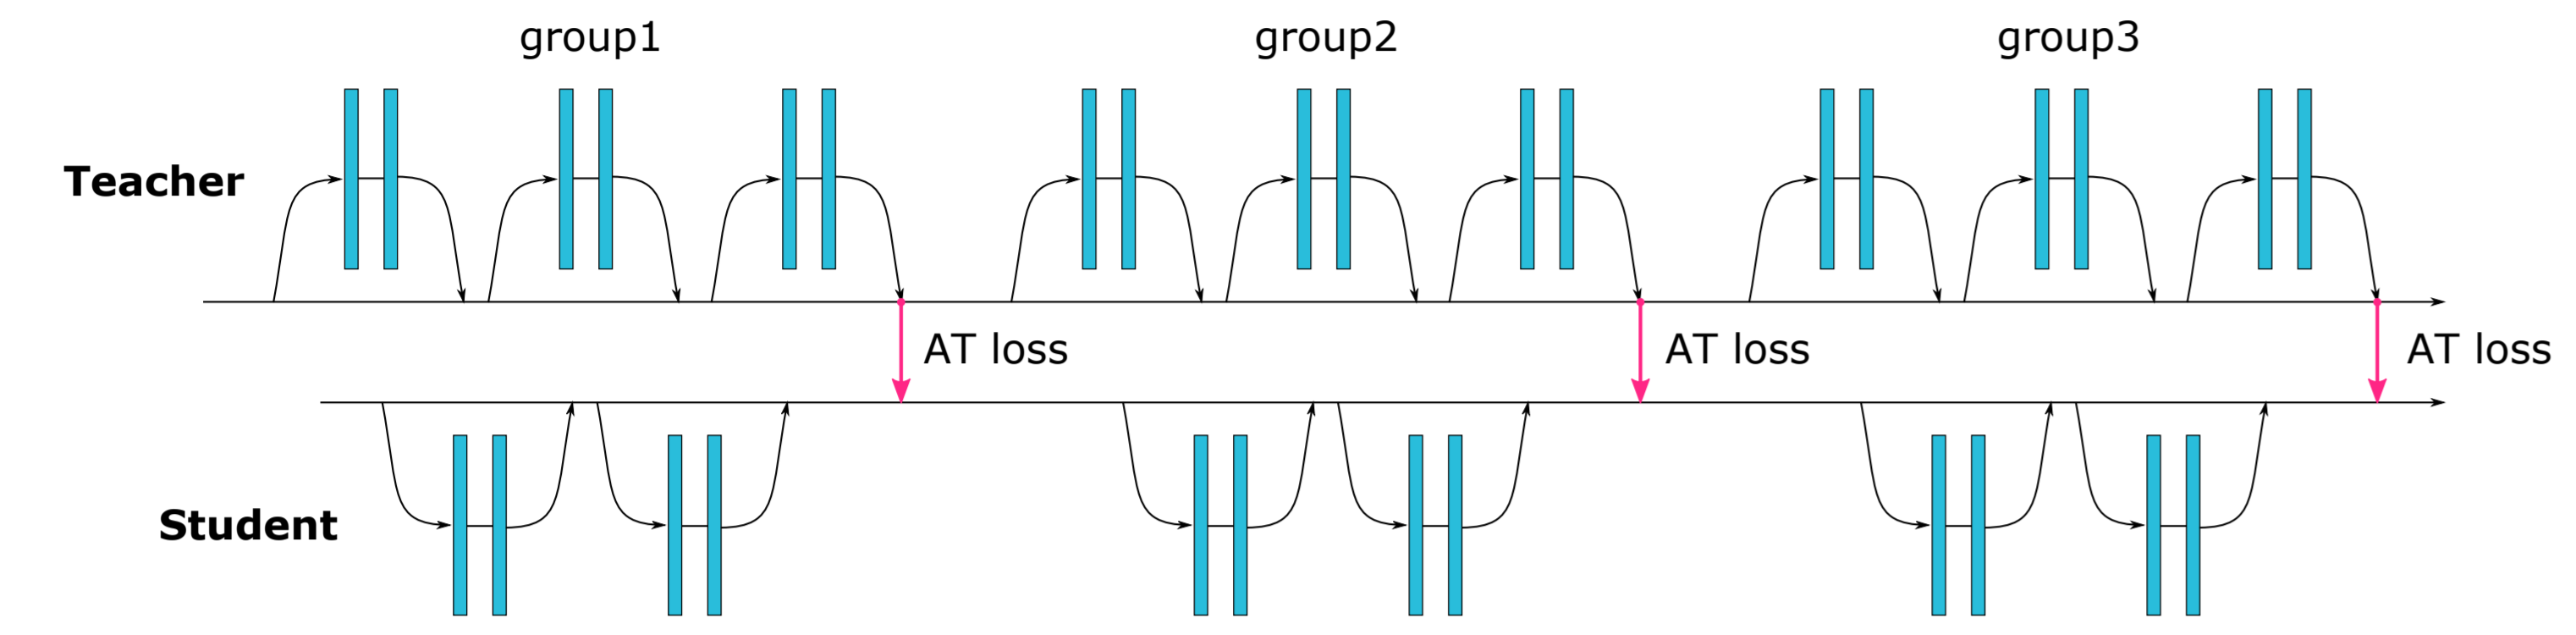
\includegraphics[width=0.8\textwidth]{att_kd.png}
\end{frame}

\begin{frame}
\frametitle{Relation Between Instances}
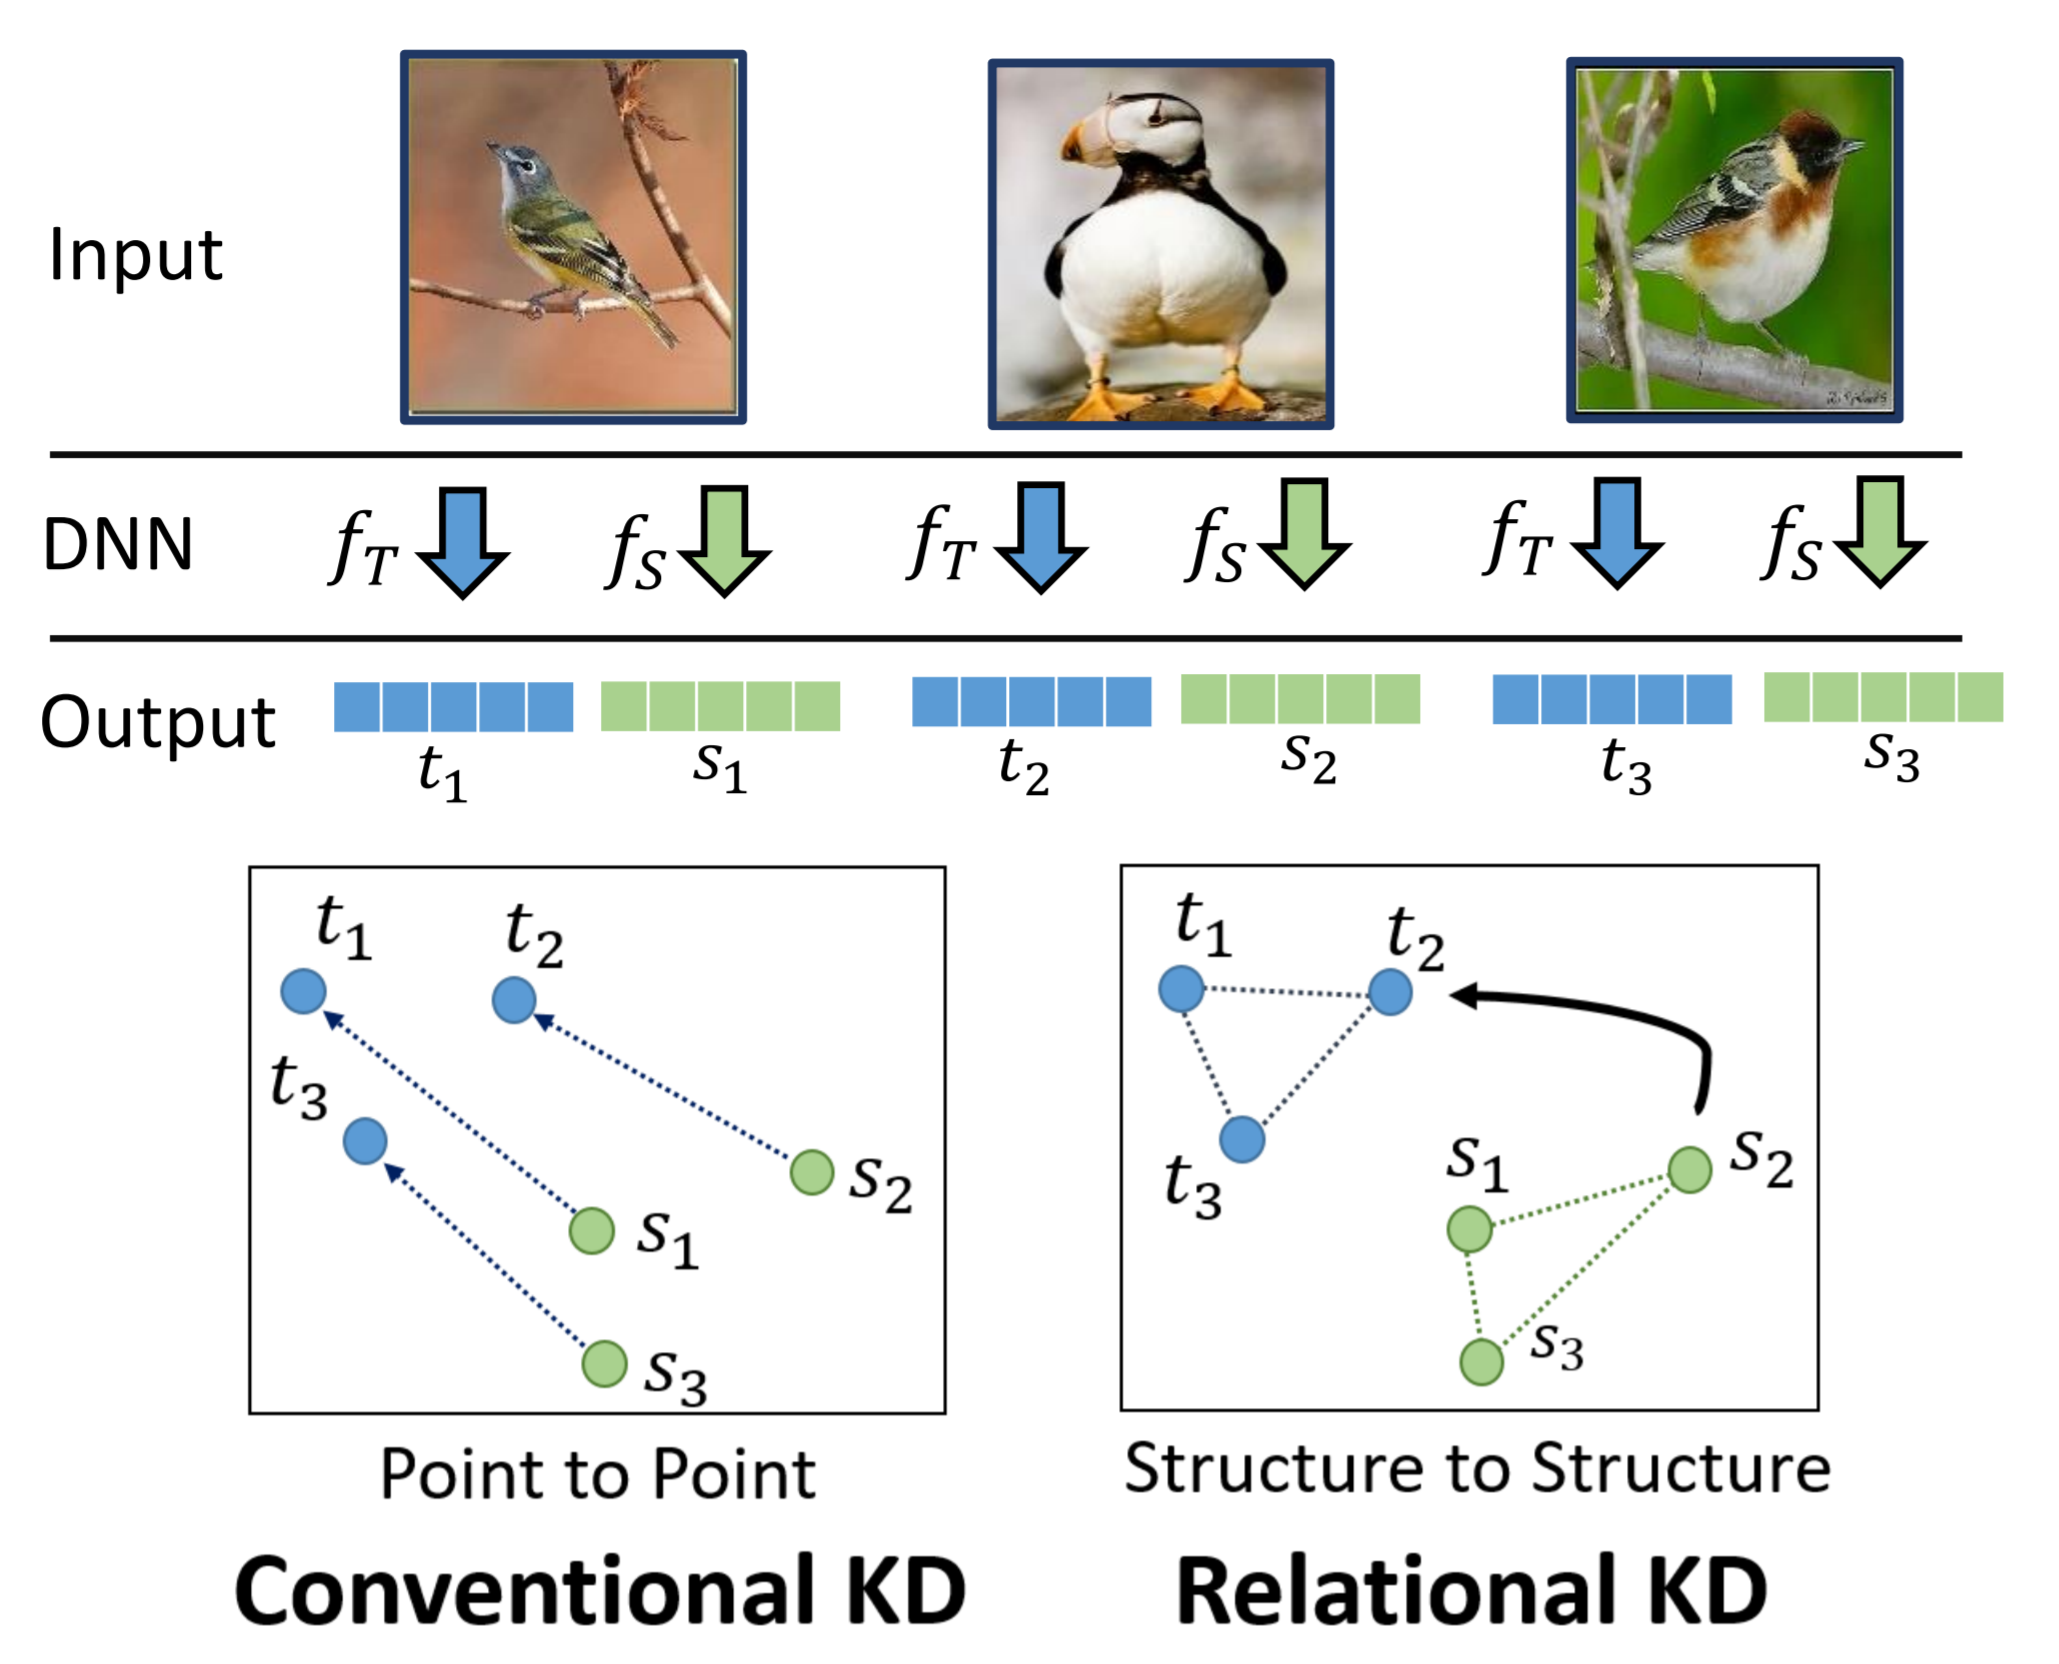
\includegraphics[width=1.0\textwidth]{structure.png}
\end{frame}

\begin{frame}
\frametitle{(CVPR2019)Relational Knowledge Distillation}
$t_i=f_T(x_i), s_i=f_S(x_i)$, $l_\delta$ is Huber loss
$L_{RKD}=\sum\limits_{(x_1,...,x_n)\in\mathcal X^N}{l_\delta(\psi(t_1,...,t_n),\psi(s_1,...,s_n))}$ \\
\vspace{5mm} %5mm vertical space
Example for $n=2$:\\
$L_{\textrm{RKD}}=\sum\limits_{(x_i,x_j)\in\mathcal X^2}{l_\delta(\psi(t_i,t_j),\psi(s_i,s_j))}$
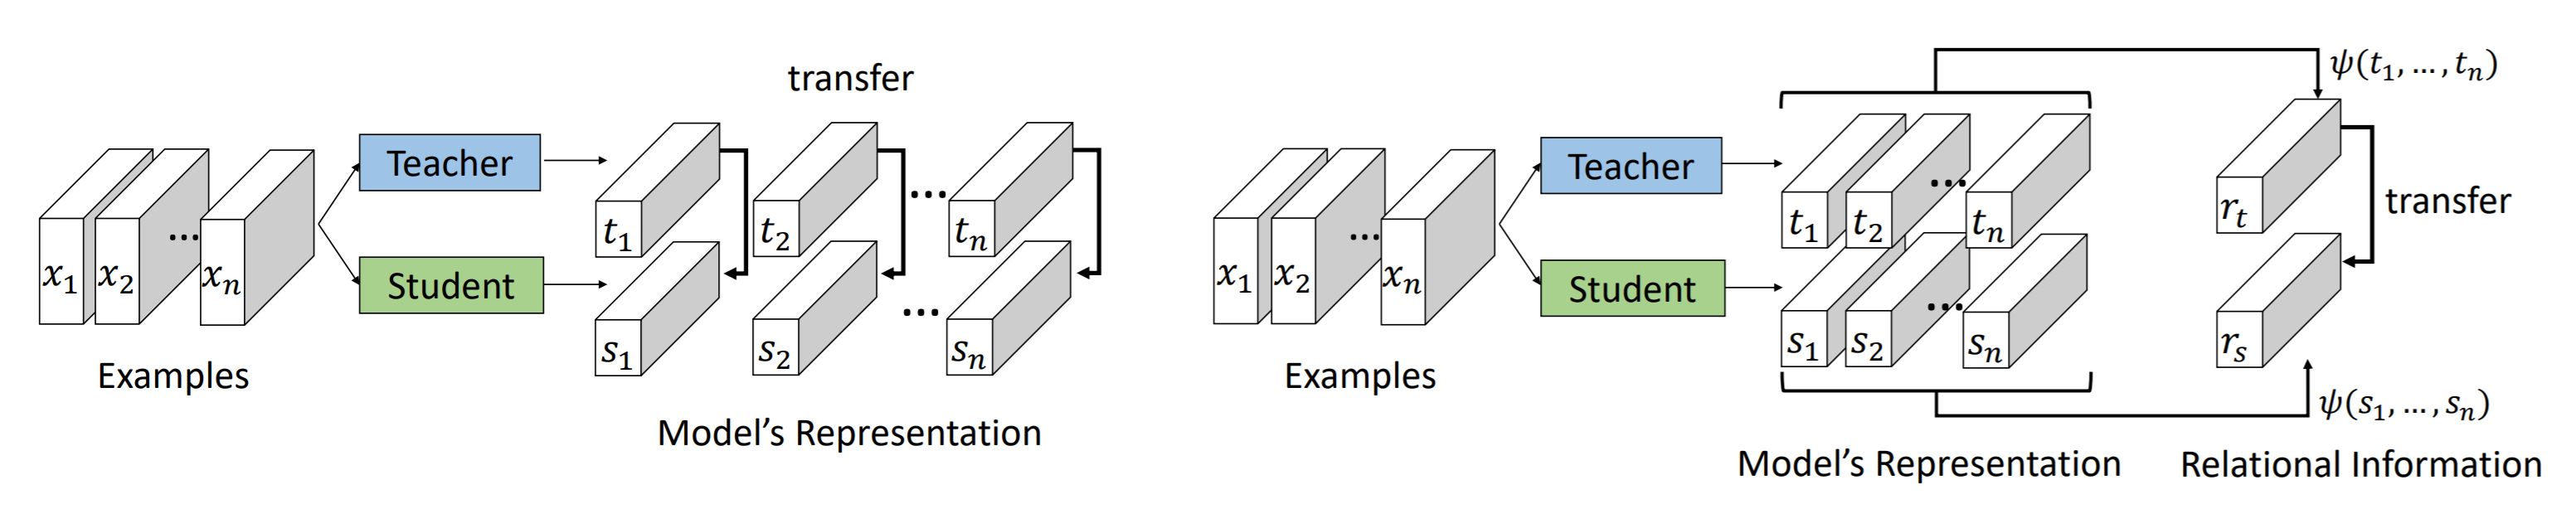
\includegraphics[width=0.8\textwidth]{rkd.png} \\
\end{frame}

\begin{frame}
\frametitle{RKD}
Distance Loss \\ $n=2,\psi_D(t_i,t_j)=\frac{1}{\mu}\|t_i-t_j\|_2$ \\
$\mu=\frac{1}{|\mathcal X^2|}\sum\limits_{(x_i,x_j)\in \mathcal X^2}\|t_i-t_j\|_2$\\
$L_{\textrm{RKD-D}}=\sum\limits_{(x_i,x_j)\in\mathcal X^2}{l_\delta(\psi_D(t_i,t_j),\psi_D(s_i,s_j))}$ \\
\vspace{5mm} %5mm vertical space
Angle Loss \\ $n=3,\psi_A(t_i,t_j, t_k)=\cos\angle{t_it_jt_k}=\langle\bm e^{ij}, \bm e^{kj}\rangle$\\
where $\bm e^{ij}=\frac{t_i-t_j}{\|t_i-t_j\|_2},\bm e^{kj}=\frac{t_k-t_j}{\|t_k-t_j\|_2}$
$L_{\textrm{RKD-A}}=\sum\limits_{(x_i,x_j, x_k)\in\mathcal X^3}{l_\delta(\psi_D(t_i,t_j, t_k),\psi_D(s_i, s_j, s_k))}$
\end{frame}

\begin{frame}
\frametitle{RKD}
Use RKD alone. \\
$L=L_{\textrm{GT}}+\lambda_{\textrm{D}}L_{RKD-D}(+\lambda_{\textrm{A}}L_{RKD-A})$\\
Use RKD with vanilla KD. \\
$L=L_{\textrm{GT}}+L_{\textrm{KD}}+\lambda_{\textrm{D}}L_{RKD-D}(+\lambda_{\textrm{A}}L_{RKD-A})$
\end{frame}

\begin{frame}
\frametitle{(CVPR2019)Knowledge Distillation via Instance Relationship Graph}
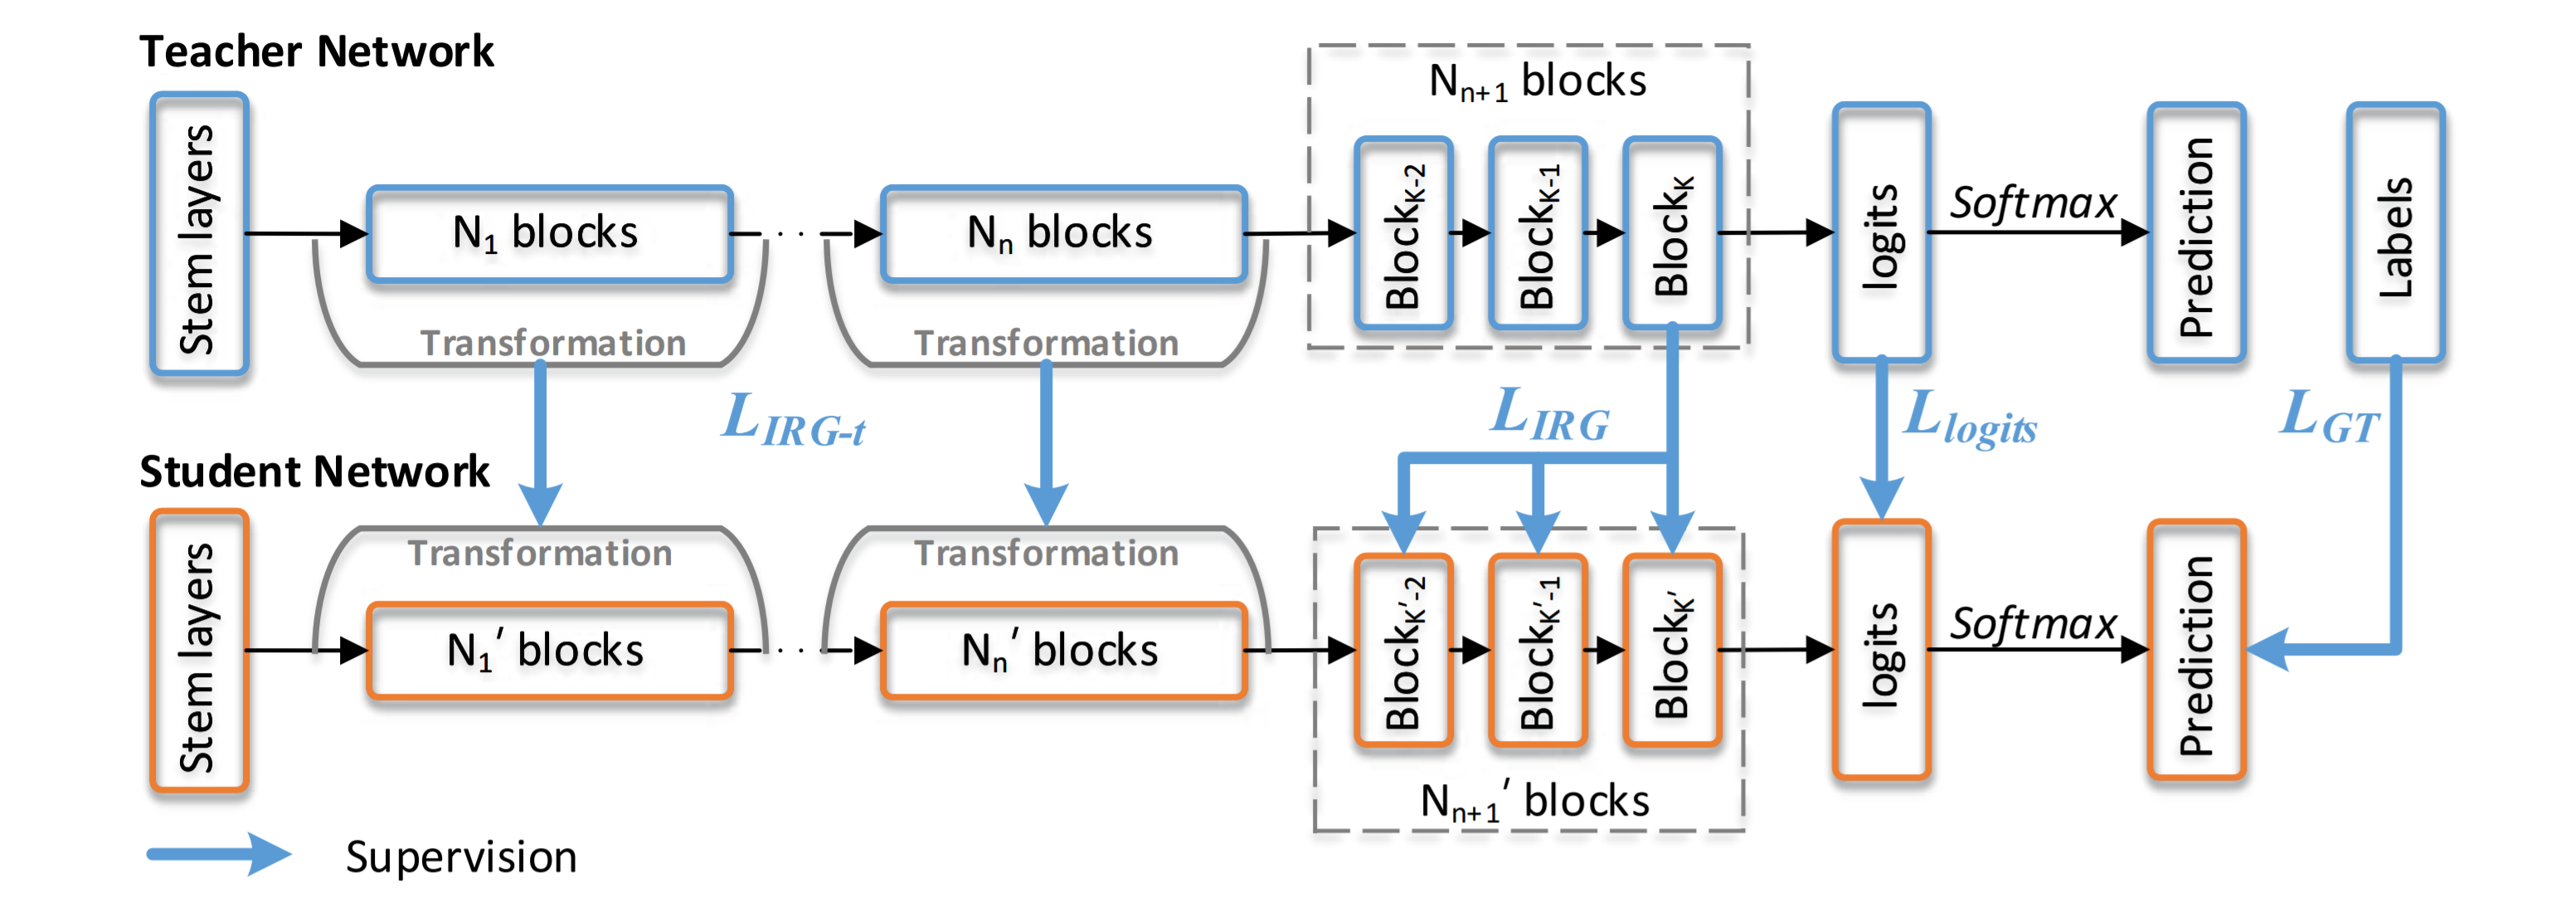
\includegraphics[width=1.0\textwidth]{irg.png}
Instance Relationship Graph of $l$-th layer:\\
Vertex $i$: $f_l(x_i)$ \\
Edge $(i,j)$: $\bm A_{l}(i, j)=\|f_l(x_i)-f_l(x_j)\|_2^2$ \\
\end{frame}

\begin{frame}
\frametitle{IRG}
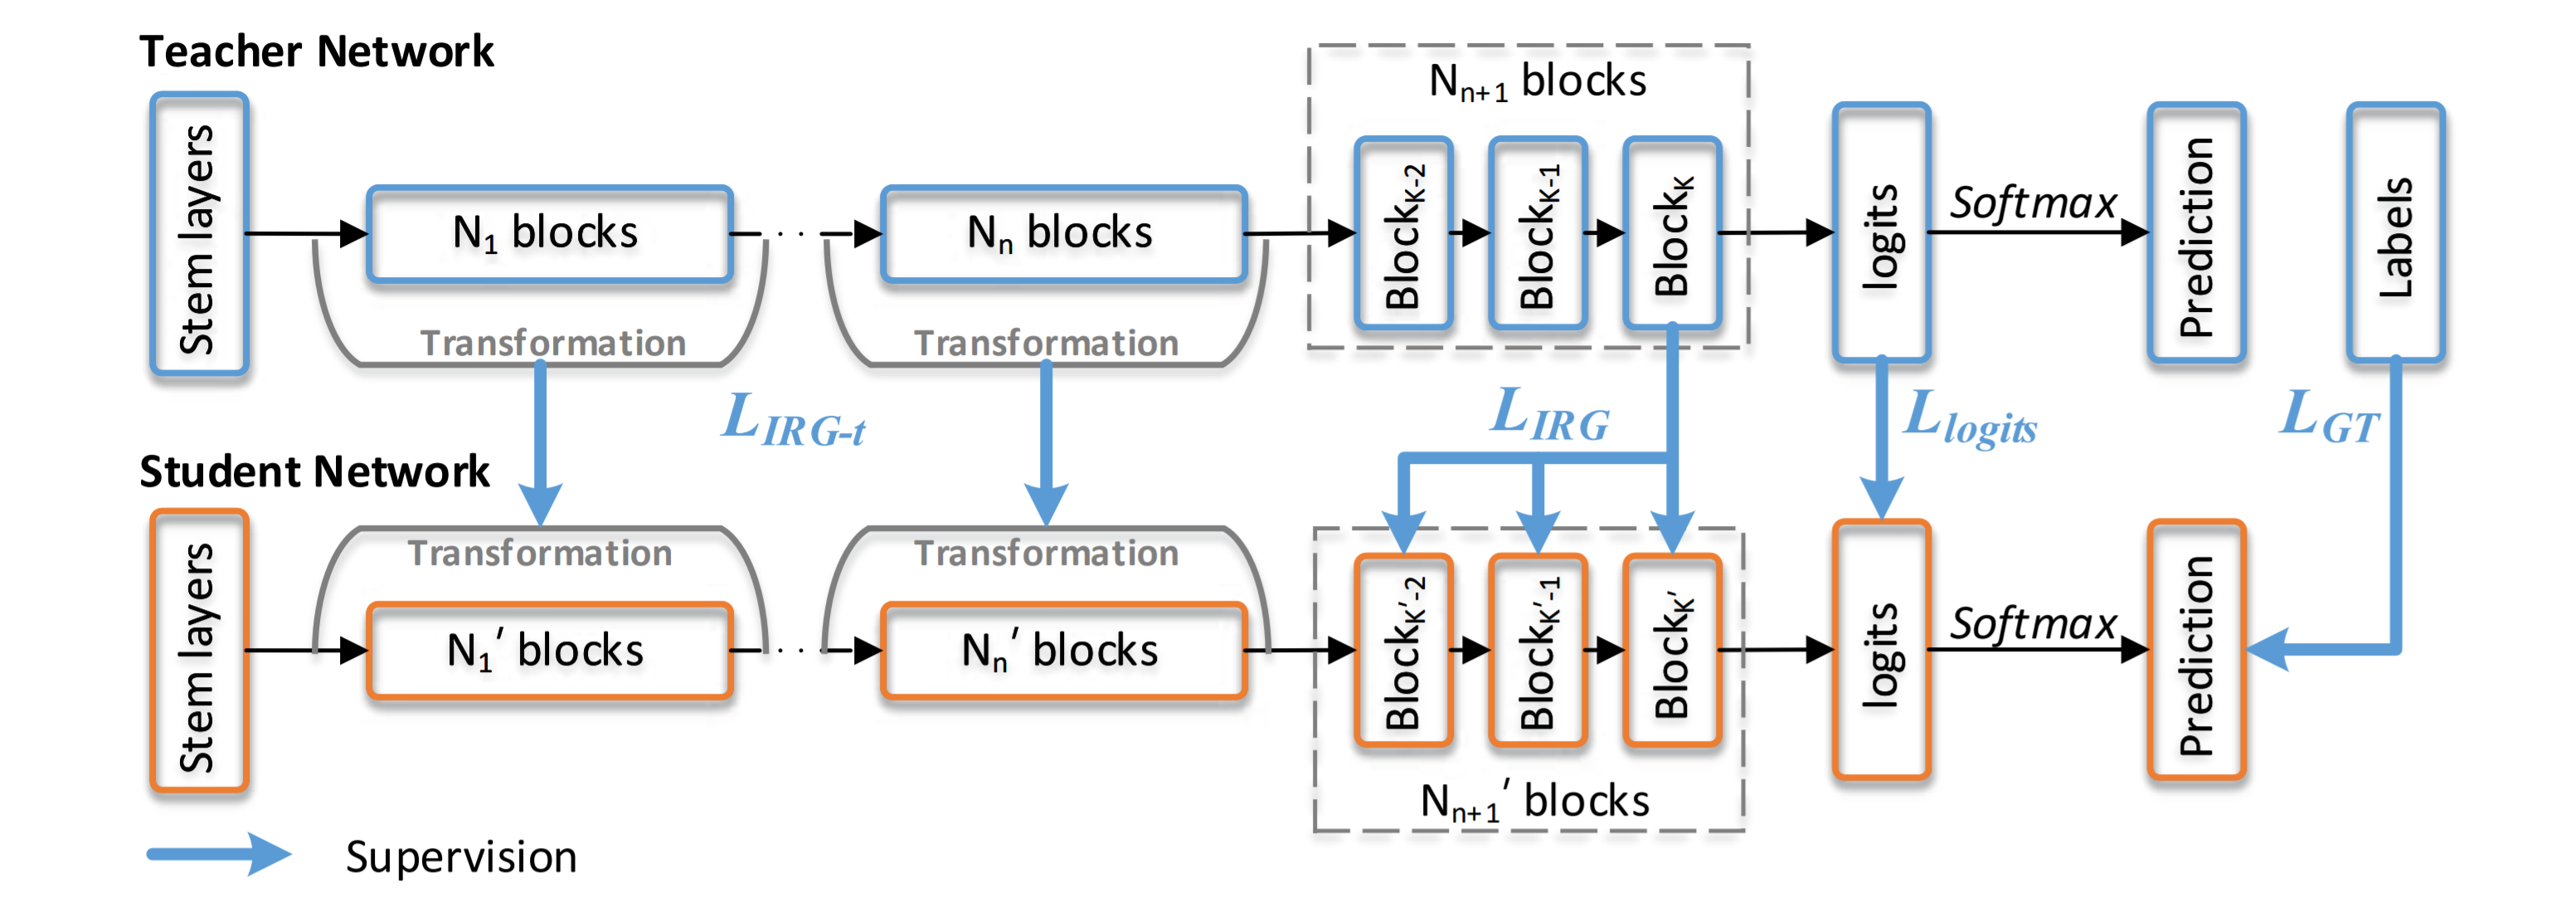
\includegraphics[width=1.0\textwidth]{irg.png}
Graph Loss:\\
$L_{\textrm{IRG}}(\bm x)=\lambda_1\sum\limits_{i=1}^I\|f^T_L(x_i)-f^S_{l_M}(x_i)\|_2^2+\lambda_2\|\bm A^T_L-\bm A^S_{l_M}\|_2^2$ \\
\end{frame}

\begin{frame}
\frametitle{IRG}
Graph Transformation from $l_1$-th layer to $l_2$-th layer:\\
Vertex Transformation: $\bm \Lambda_{l_1,l_2}(i, i)=\|f_{l_1}(x_i)-f_{l_2}(x_i)\|_2^2$\\
Edge Transformation: $\bm \Omega_{l_1,l_2}=\|\bm A_{l_1}-\bm A_{l_2}\|_2^2$ \\
\vspace{5mm}
Graph Transformation Loss:\\
$L_{\textrm{IRG-t}}(\bm x)=\|\bm \Lambda^T_{l_1,l_2}-\bm \Lambda^S_{l_3,l_4}\|_2^2+\|\bm \Omega^T_{l_1,l_2}-\bm \Omega^S_{l_3,l_4}\|_2^2$ \\


\end{frame}

\begin{frame}
    \frametitle{IRG}
    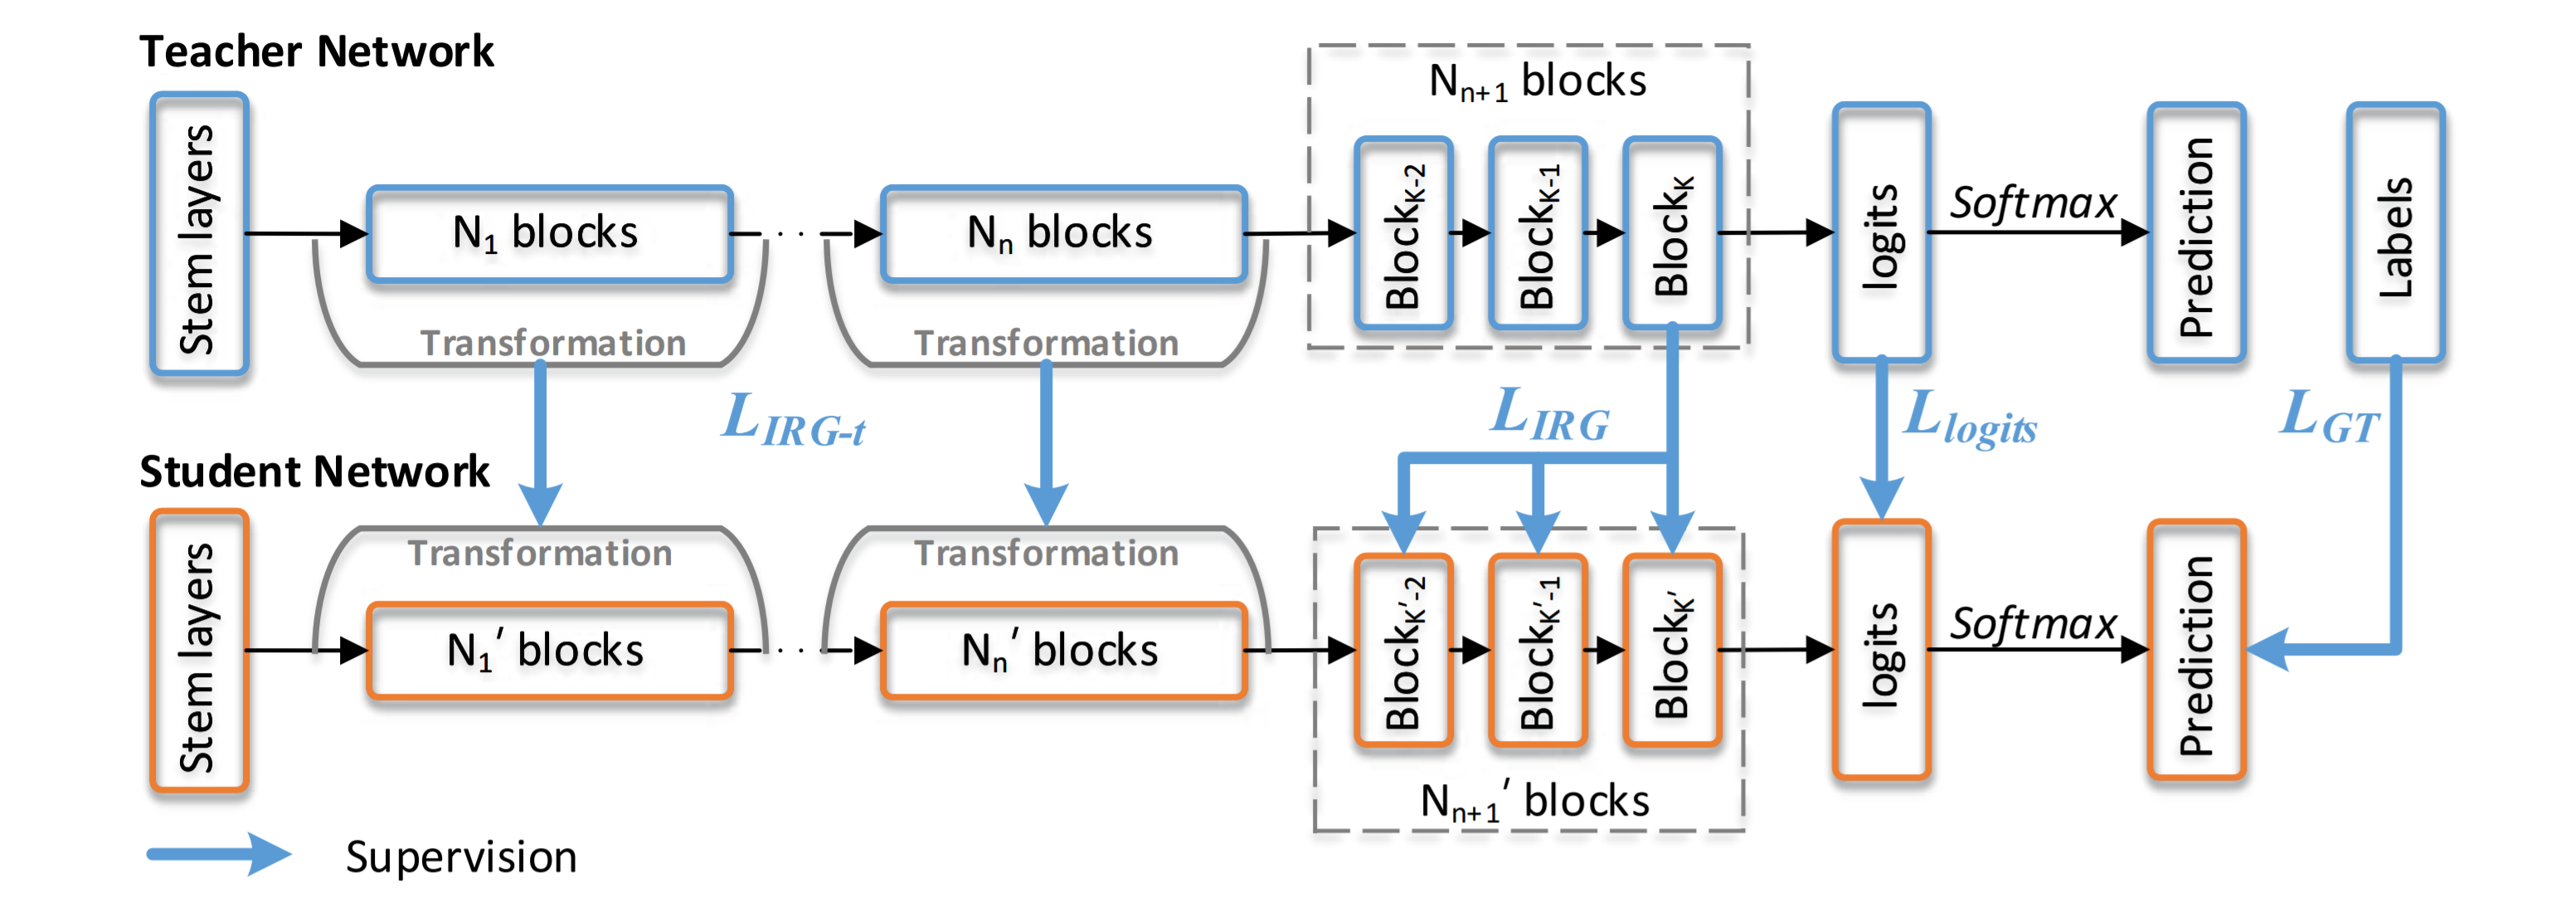
\includegraphics[width=1.0\textwidth]{irg.png}
    $L_{MTK}(\bm x)=L_{GT}(\bm x)+\lambda_1L_{logits}(\bm x) + \lambda_2\sum\limits_{l_M\in \bm{L_M}}\|\bm A_L^T-\bm A_{l_M}^S\|_2^2+\lambda_3\sum\limits_{l_1l_2l_3l_4\in \bm{L_{Trans}}}{\|\bm \Lambda_{l_1,l_2}^T-\bm \Lambda_{l_3,l_4}^S\|_2^2}$ \\
\end{frame}

\begin{frame}
    \frametitle{(ICCV2019)Correlation Congruence for Knowledge Distillation}
    $k(\bm x, \bm y)=exp(-\frac{\|\bm x-\bm y\|_2^2}{2\delta^2})$\\
    $[k(\bm F, \bm F)]_{ij}=exp(-\gamma\|\bm F_i-\bm F_j\|^2) \approx \sum_{p=0}^P{exp(-2\gamma)\frac{(2\gamma)^p}{p!}(\bm F_i \bm F_j^T)^p}$
\end{frame}

\begin{frame}
    \frametitle{(ICCV2019)Correlation Congruence for Knowledge Distillation}
    There is intra-class bias in minibatch.\\
    CUR-sampler: $m$ classes, $m*k$ samples.\\
    SUR-sampler: do k-means first.(superclass)\\
    \vspace{8mm}
    The other two papers do not mention this problem.
\end{frame}

\begin{frame}
    \frametitle{Summary}
    Use information between instances. \\
    Can be used in hidden layer. \\
    \vspace{8mm}
    Other form of distance/correlation between instances. (ICLR 2020, Contrastive Representation Distillation) \\
    Which layers to match between teacher and students?
\end{frame}


\end{document}
